\section{Análisis de Resultados}

Se pudo ver que ambas arquitecturas presentan características y ventajas distintas. 
La arquitectura Kappa es la más adecuada para procesar datos en tiempo real, con muy baja latencia. 
Como contraparte presenta un uso de recursos más elevado que Delta y una mayor complejidad operativa.

Por su lado, Delta parece ser más escalable con menos recursos, 
ya que puede ingestar una mayor cantidad de datos en la misma cantidad de tiempo.
Sin embargo, sus tiempos de latencia lo hacen inadecuado para procesamiento en tiempo real. 

Considerando esto, si el objetivo del sistema es el monitoreo de pacientes ambulatorios por ejemplo, 
la arquitectura Delta es más adecuada, ya que no necesariamente requiere un accionar del sistema de forma inmediata.

En cambio, si el objetivo es el monitoreo de pacientes en una sala de emergencias o cuidados intensivos,
la arquitectura Kappa es la más adecuada, ya que permite actuar de forma inmediata ante cualquier evento inesperado.

Para un sistema de salud integral, se podrían combinar ambas arquitecturas, 
utilizando Delta como fuente de verdad, y un subsistema basado en Kappa para el monitoreo intrahospitalario,
donde la latencia es crítica. 
Este subsistema podría a su vez alimentar al sistema principal de modo que todos los datos fluyan por ambos.

Esta idea es similar a la arquitectura Lambda, aunque optimizado para el procesamiento continuo de datos.
Lo más interesante de este enfoque es que se puede hacer con las tecnologías actuales,
Kafka seguiría siendo el punto de ingesta de datos, 
luego cada uno de los sistemas podrías hacer su análisis. Por último Kappa enviaría sus datos a Doris, 
que además ya está configurado para poder hacer las consultas federadas sobre los datos que almacena Delta. 
Esto permitiría tener un sistema de salud integral, 
donde consultar datos en tiempo real, que pueden tener un ciclo de vida corto que permita el menor uso de recursos 
y a su vez consultar los datos históricos que fueron procesados de manera contínua pero que tienen una latencia de 
algunos minutos. 

\begin{figure}
    \centering
    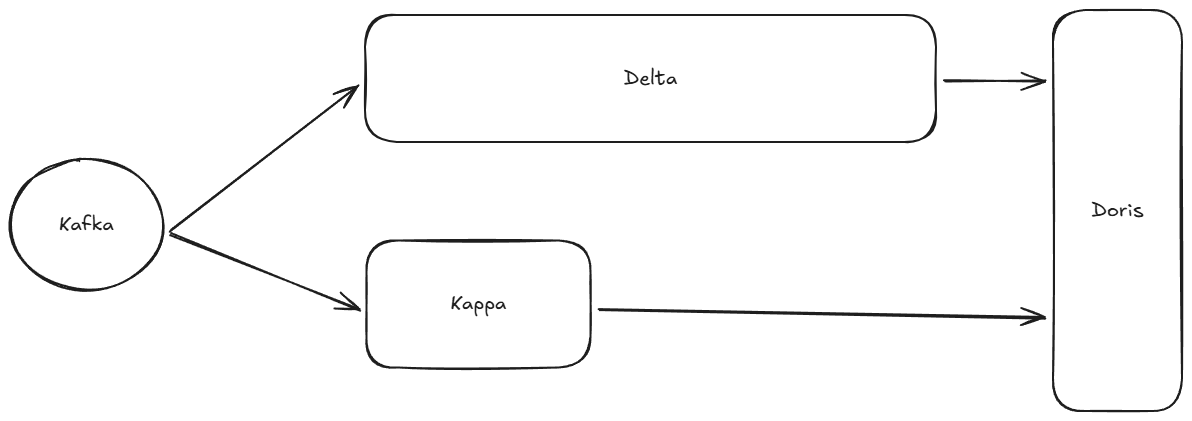
\includegraphics[width=0.8\textwidth]{resultados/combine.png}
    \caption{Arquitectura de un sistema integral de salud}
    \label{fig:analisis}
\end{figure}